\newpage
\section{Veretiefungsprojekt: Q-Learning mit OpenAI Gym}
\label{section:q-learning-vertiefung}
Zur Vertiefung des Kapitels wurde das Q-Learning mit Python und OpenAI Gym implementiert. Die Umsetzung erfolgte auf der Grundlage eines Online-Artikels von learndatasci.com\cite{q-learning-article}. In diesem Beispiel wurde die OpenAI Gym-Umgebung ``Taxi-v3'' verwendet, die die Zust�nde, Aktionen und Belohnungen f�r den Q-Learning-Algorithmus und das Rendering der Zustandsdarstellung bereitstellt. Der vollst�ndige Code des Programms ist unter vertiefungen-projekte/python/reinforcement-learning/ zu finden.

\begin{figure}[H]
    \centering
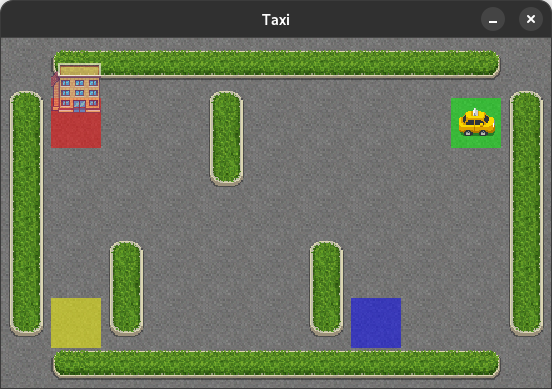
\includegraphics[width=0.7\textwidth]{figures/kap14/vertiefung-qlearning.png}
    \caption{Screenshot der trainierten KI}
    \label{fig:q-learning-screenshot}
\end{figure}

\subsection{Ausf�hren des Programms}
Um das Programm auszuf�hren:
\begin{enumerate}
    \item Zum Ordner navigieren: vertiefungen-projekte/python/reinforcement-learning/
    \item F�hre Folgendes in einem Terminal aus
\begin{lstlisting}[language=bash]
# install dependencies
pip install -r requirements.txt

# run program
python3 taxi-qlearning.py
\end{lstlisting}
\end{enumerate}

\subsection{�berblick �ber den Ablauf}
Das Programm beginnt mit der Erstellung der OpenAI Gym-Umgebung und der Initialisierung einer leeren Q-Tabelle. Das Programm beginnt mit der Erstellung der OpenAI Gym-Umgebung und der Initialisierung einer leeren Q-Tabelle.

\begin{lstlisting}[language=python]
env = gym.make("Taxi-v3").env
q_table = np.zeros([env.observation_space.n,env.action_space.n])
\end{lstlisting}

Die Parameter f�r die Q-Regel werden dann wie folgt festgelegt.

\begin{lstlisting}[language=python]
# Q-Regel parameters
alpha = 0.1
gamma = 0.6
epsilon = 0.1
\end{lstlisting}

Das Training beginnt dann f�r jede Epoche in der While-Schleife. Zu Beginn einer Epoche wird ein zuf�lliger Wert gegen Epsilon gepr�ft, um zu entscheiden, ob der Aktionsraum erkundet oder bereits erlernte Werte ausgenutzt werden sollen.

\begin{lstlisting}[language=python]
while not epoch_done:
if random.uniform(0, 1) < epsilon:
    action = env.action_space.sample() # Explore action space
else:
    action = np.argmax(q_table[state]) # Exploit learned values
\end{lstlisting}

Dann wird eine Aktion durchgef�hrt (entweder aus der Q-Tabelle oder aus der Umgebung) und die Q-Tabelle wird unter Verwendung der Q-Regelgleichung aktualisiert.

\begin{lstlisting}[language=python]
next_state, reward, epoch_done, info = env.step(action) 

old_value = q_table[state, action]
next_max = np.max(q_table[next_state])

new_value = (1 - alpha) * old_value + alpha * (reward + gamma * next_max)
q_table[state, action] = new_value
\end{lstlisting}

Dies wird f�r jede Epoche in jeder Episode durchgef�hrt, bis das Training abgeschlossen ist. Schlie�lich wird das trainierte Modell getestet (und gerendert), um zu beobachten, wie gut es trainiert wurde. 